از آنجایی که ضخامت غشا از مرتبه‌ی چند نانومتر و اندازه‌ی آن حدود چند میکرون است می‌توانیم از مدل‌های الاستیک پوسته‌های نازک برای مطالعه رفتار مکانیکی آن استفاده کنیم. در این رژیم فرض می‌کنیم که غشا یک لایه‌ی نازک است که در تقریب مقیاس طولی بزرگ (چند میکرون) مساحت ثابتی دارد. توصیف پوسته‌های نازک را با بررسی انرژی خمشی و انرژی کششی یک محیط پیوسته آغاز خواهیم کرد. پس حل معادلات پیوسته، این معادلات را برای مجموعه نقاط در فضا که بر روی شبکه‌ی مثلثی قرار دارند حل می‌کنیم. سپس تغییرات انرژی در صورت ایجاد نقاط نقص بر روی شبکه را محاسبه خواهیم کرد. 


%مقاله الکساندرا مرجع ۷ در مقده تيوری خیلی خوب راجع به آنالیز فرکانس نوشته


\begin{figure}[h]
\begin{center}
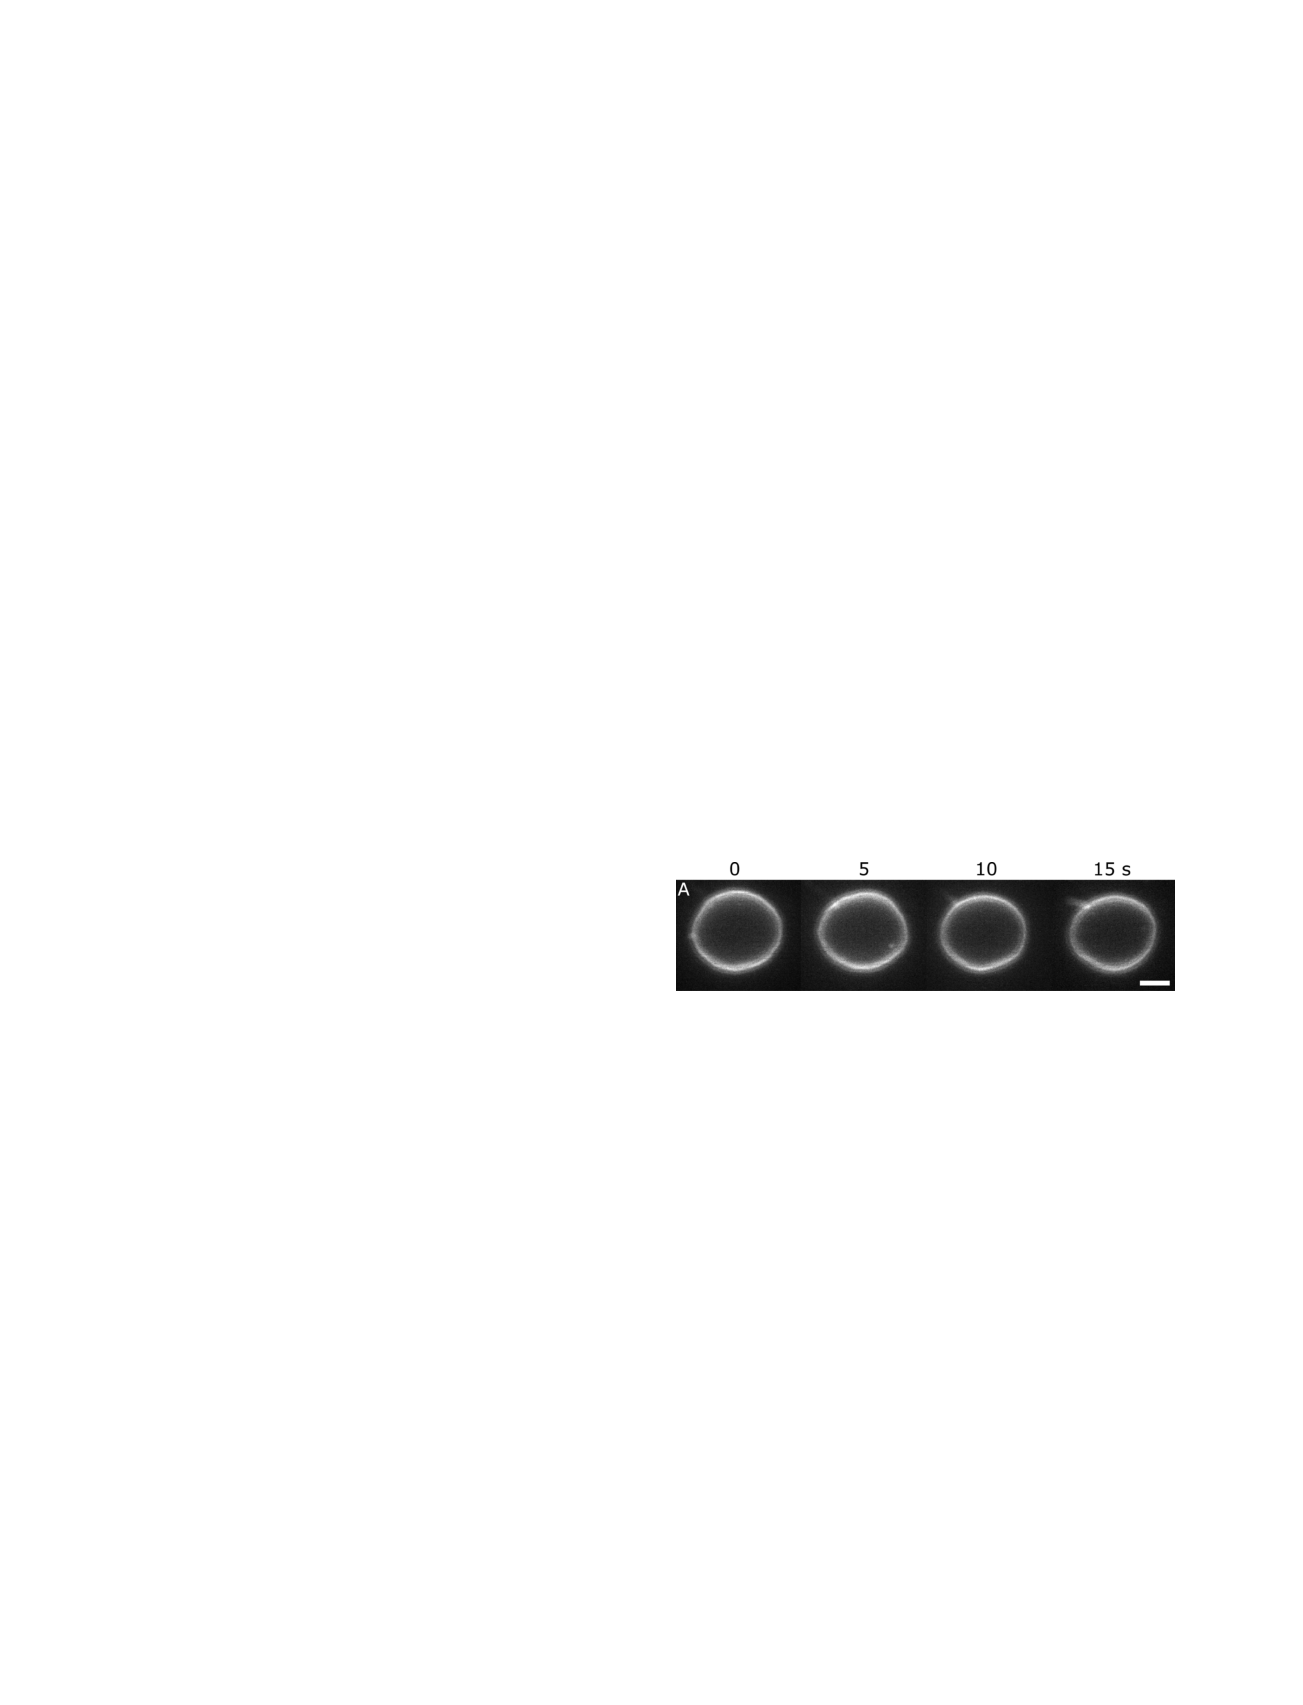
\includegraphics[width=\columnwidth]{\MemDiscr/Pics/Membrane_fluctuations}
\caption{
مجموعه تصاویر پست سر هم از تغییر شکل یک غشای لیپیدی را با تصویر برداری فلورسانت در بازه‌های ۵ ثانیه‌ای نشان می‌دهد. خط مقیاس سفید رنگ اندازه‌ی ۵ میکرومتر را نشان می‌دهد 
\cite{ParthasarathyMembraneMeasurement}.
}
\label{fig:flucmem}
\end{center}
\end{figure}

شگل 
\ref{fig:flucmem}
تغییر شکل یک غشای لیپیدی غول آسا (قطر حدود ۱۰ میکرون) در بازه‌های زمانی ۵ ثانیه نشان می‌دهد
\cite{ParthasarathyMembraneMeasurement}.
 از نظر انرژی تغییر شکل این غشا را می‌توان به دو بخش کلی تقسیم کرد. تغییر انرژی ناشی از خم شدن و تغییر حاصل از کشش سطح غشا. شکل
\ref{fig:elasticdeformation}
الف، تغییر شکل یک عنصر سطحی بر اثر خمش را نشان می‌دهد. خمش سطح را می‌توان با اندازه‌ی شعاع دو دایره که بر عنصر سطح مماس هست، توصیف کرد. همچنین شکل 
\ref{fig:elasticdeformation}
ب، تغییر شکل عنصر سطح به علت ایجاد کشش در سطح نشان می‌دهد. تغییر سطح با اختلاف مساحت عنصر سطح با حالت کشیده نشده توصیف می‌شود.
\begin{figure}[h]
\begin{center}
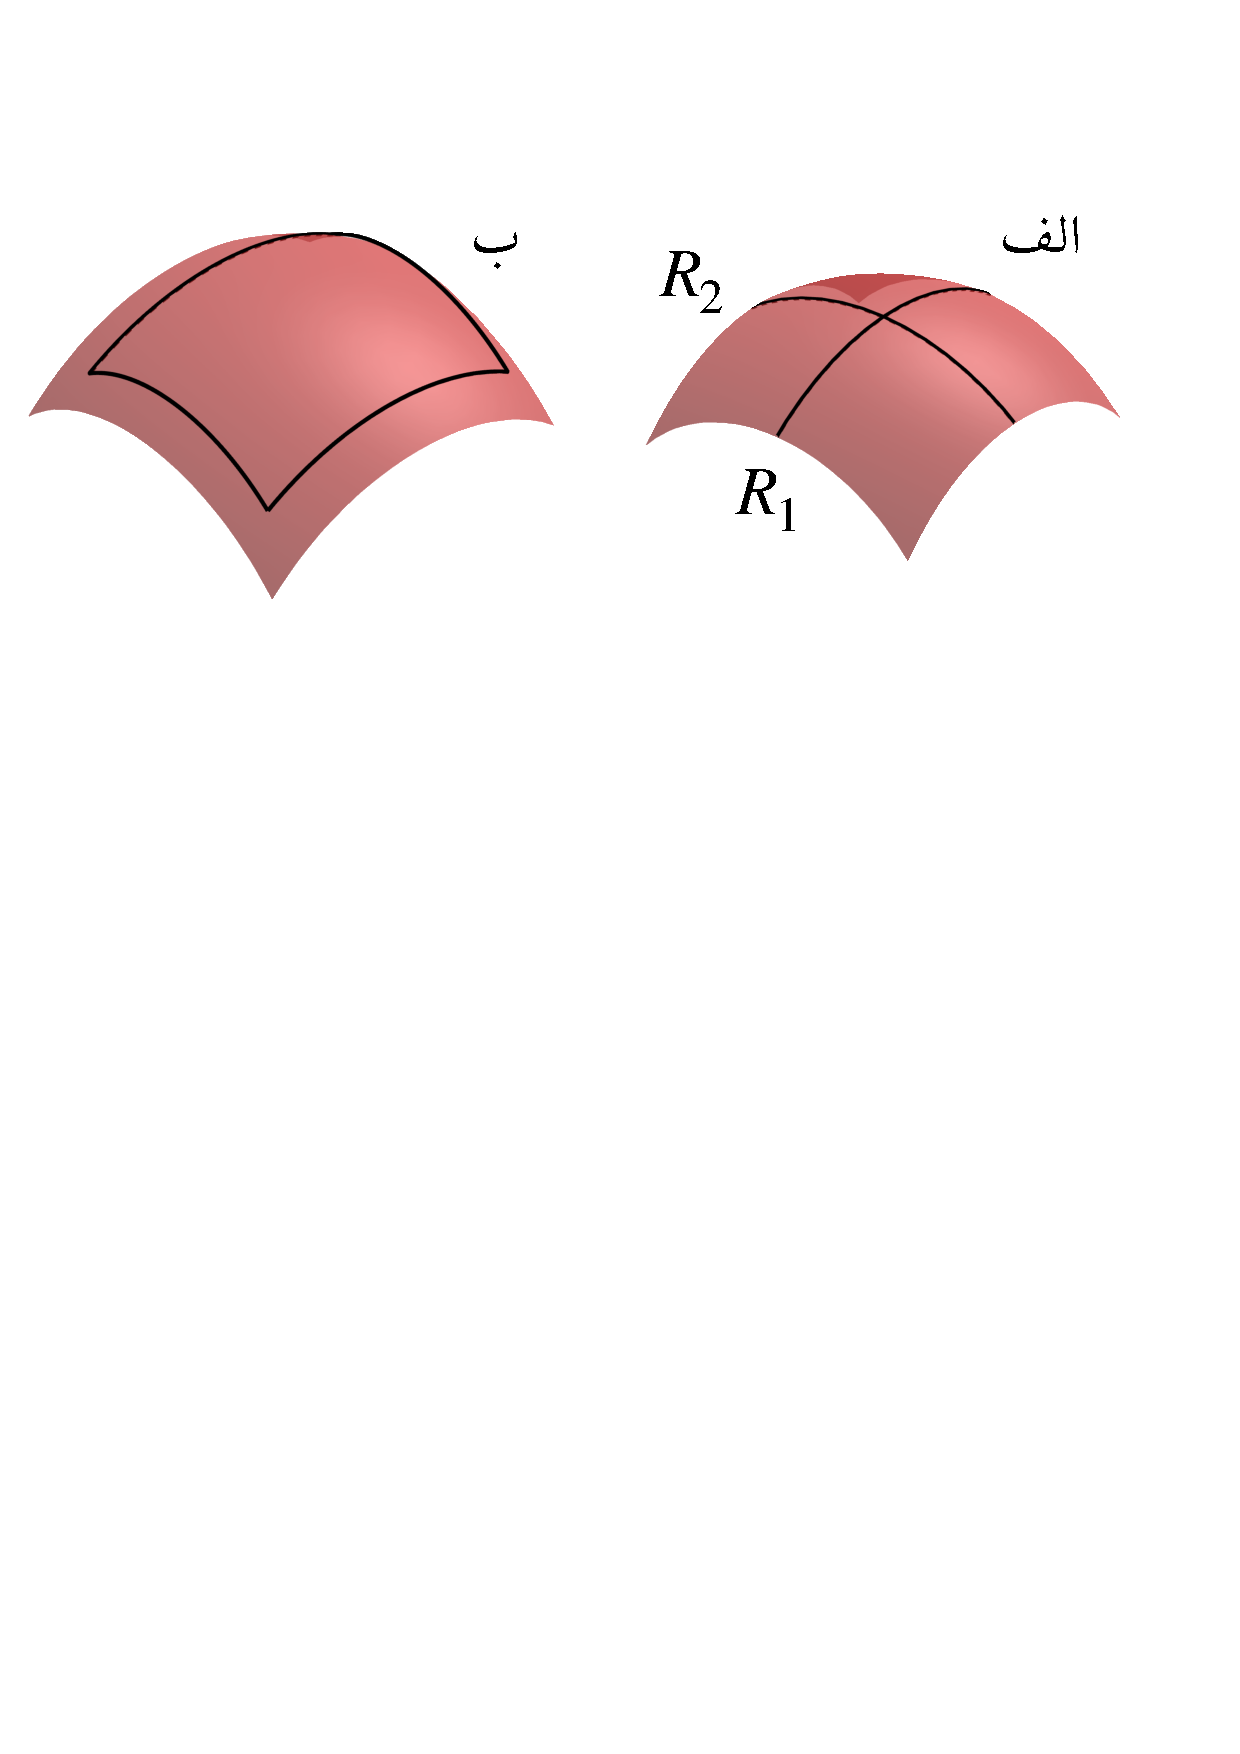
\includegraphics[width=\columnwidth]{\MemDiscr/Pics/surface elemnts.pages.pdf}
\caption{
تغییر شکل عنصر سطحی بر اثر الف، خمش و ب، کشش.
}
\label{fig:elasticdeformation}
\end{center}
\end{figure}




